\documentclass[border=20pt]{standalone}
\renewcommand\familydefault{\sfdefault} % Default family: serif 
\usepackage[usenames,dvipsnames]{xcolor}
\usepackage{tikz}
%\usepackage{soul}
\usetikzlibrary{calc} 
\usetikzlibrary{arrows, decorations.markings,positioning,backgrounds,shapes}
\usetikzlibrary{patterns}
\usetikzlibrary{fit}
\usepackage[normalem]{ulem}

\begin{document}
	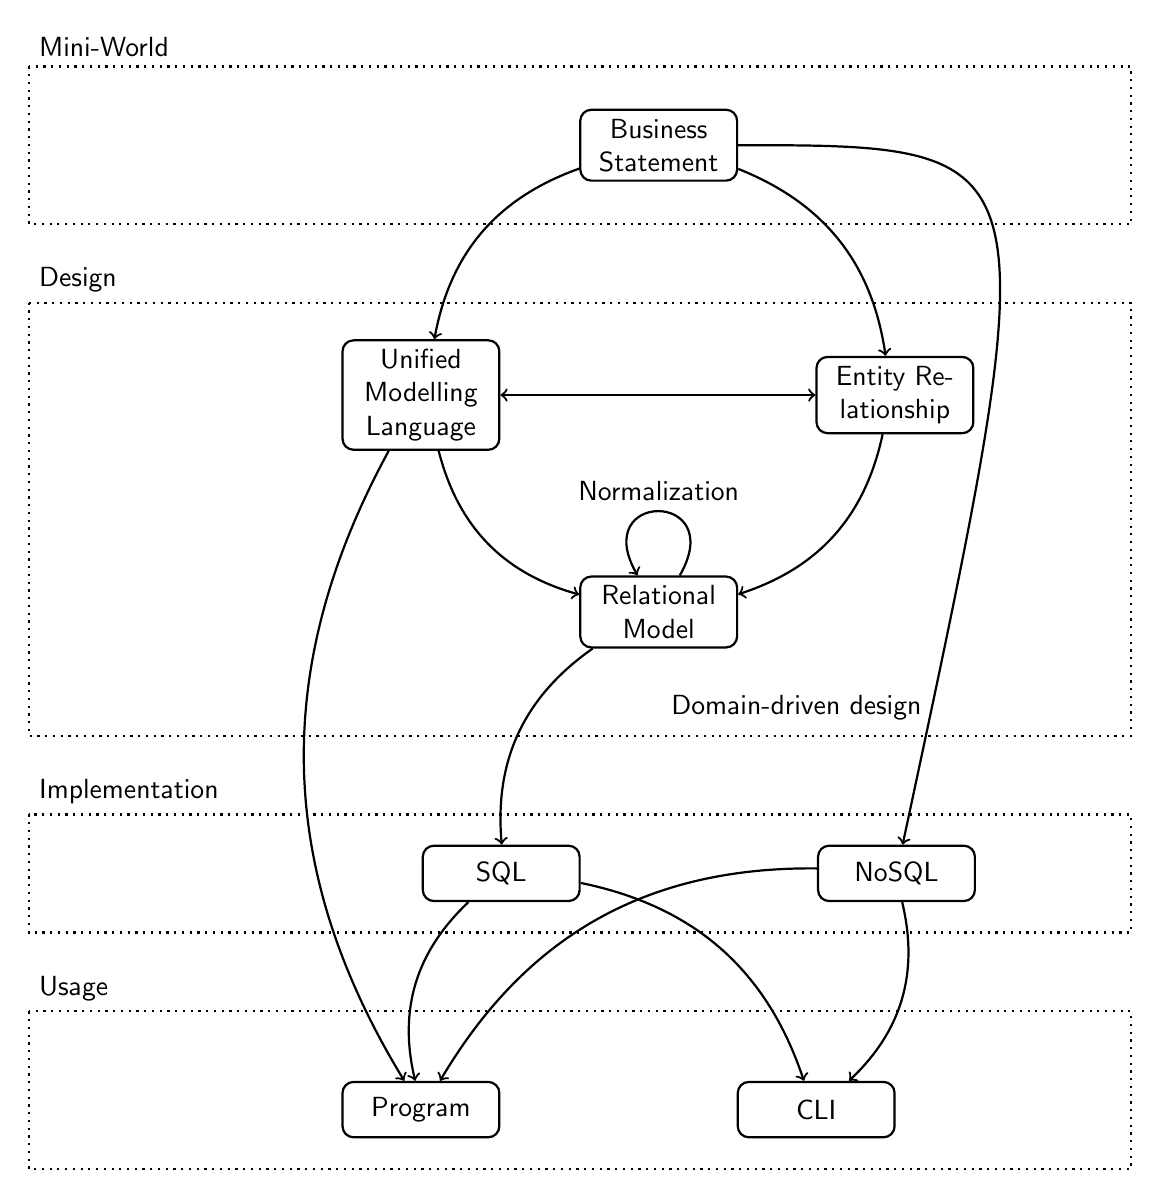
\begin{tikzpicture}[ 
    block/.style={
      rectangle,
      thick,
      text width=5em,
      align=center,
      rounded corners,
      minimum height=2em
    },
	data/.style={
		cylinder,
		draw=black,
		thick,
		aspect=0.7,
		minimum height=1.7cm,
		minimum width=1.5cm,
		shape border rotate=90,
		cylinder uses custom fill,
		cylinder body fill=red!30,
		cylinder end fill=red!10
	}
]

%\node (caption) at (-1.5,2) {In \textcolor{green}{green}, the DBMS software.};

\node [block, draw=black] (business) at (0,0) {Business Statement};
\node [block, draw=black] (uml) [below left = 2cm and 1cm of business] {Unified Modelling Language};
\node [block, draw=black] (er) [right = 4cm of uml] {Entity Relationship};
\node [block, draw=black] (rel) [below = 5cm of business] {Relational Model};
\node [block, draw=black] (sql) [below right = 5cm and -1cm of uml] {SQL};
\node [block, draw=black] (nosql) [right = 3cm of sql] {NoSQL};
\node [block, draw=black] (prog) [below = 8cm of uml] {Program};
\node [block, draw=black] (cli) [right = 3cm of prog] {CLI};

%% Frame

\draw[thick,dotted] (-8,1) node[above right]{Mini-World} rectangle (6,-1);
\draw[thick,dotted] (-8, -2) node[above right]{Design} rectangle (6,-7.5);
\draw[thick,dotted] (-8, -8.5) node[above right]{Implementation} rectangle (6,-10);
\draw[thick,dotted] (-8, -11) node[above right]{Usage} rectangle (6,-13);


%%% Arrows
\draw [->, thick] (business) to [bend left] (er);
\draw [->, thick] (business) to [bend right] (uml);
\draw [->, thick] (er) to [bend left] (rel);
\draw [->, thick] (uml) to [bend right] (rel);
\draw [<->, thick] (er) to (uml);
\draw [->, thick] (rel) to [bend right] (sql);
\draw [->, thick] (sql) to [bend left] (cli);
\draw [->, thick] (sql) to [bend right] (prog);
\draw [->, thick] (nosql) to [bend left] (cli);
\draw [->, thick] (nosql) to [bend right] (prog);
\draw [->, thick,bend left] (business) %.. controls +(5,0) and +(4,0).. 
%-- +(8,0) -- +(8, -10) -- 
.. controls +(5,0) ..
node[left, pos=.93]{Domain-driven design} (nosql);
\draw[->, thick, every loop/.style={looseness=6}] (rel) edge  [in=120,out=60, loop, above]  node {Normalization} ();

\draw [->, thick] (uml) to [bend right] (prog);

%\draw [<->, thick] (user) to [bend right] (cli.west);
%\draw [<->, thick] (program) to [bend left] (process);
%\draw [<->, thick] (cli) to [bend right] (process);
%\draw [<->, thick] (process) to (access);
%\draw [<->, thick] (access) to (data);
%\draw [<->, thick] (access) to (metadata);

%	% Caption:
%	\node (caption) at (-5.5,2) {	Common term, \emph{CS term}, \underline{Relational Model term}, \sout{To be avoided}};
%	
%	% Table:
%	\node (name) {\textbf{STUDENT}};
%	\node [below of=name] (Name) {\textbf{Name}};
%	\node [right= 3 of Name] (dots1) {\(\cdots\)};
%	\node [right= 3 of dots1] (Major) {\textbf{Major}};
%	\node [below of= Name] (Morgan) {Morgan};
%	\node [below of= dots1] (dots2) {\(\cdots\)};
%	\node [below of= Major] (CS) {CS};
%	\node [below of= Morgan] (dots3) {\(\vdots\)};
%	\node [below of= dots2] (dots4) {\(\vdots\)};
%	\node [below of= CS] (dots5) {\(\vdots\)};
%	\node [below of= dots3] (Bob) {Bob};
%	\node [below of= dots4] (dots6) {\(\cdots\)};
%	\node [below of= dots5] (IT) {IT};
%	% Annotations:
%%	\draw [-, dashed] (-1.5, 0.75) -- ++ (11,0);
%%	\draw [-, dashed] (-1.5, -1.45) -- ++ (11,0);
%	\node (meta) at (11.2, -0.35) {\(\left.\rule{0cm}{1.2cm}\right\}\) Structure, \emph{meta-data}, \underline{schema}};
%	\node (data) at (10.4, -3.0) {\(\left.\rule{0cm}{1.65cm}\right\}\)  \emph{data}, \underline{relation state}};
%	\begin{scope}[on background layer]
%		\node [fit=(name)(IT), fill=gray!20, draw = none, inner sep= 15pt] (box1) {};	
%		\node [fit=(Name)(Major), fill=blue!20, draw = none, inner sep= 5pt] (box2) {};	
%		\node [fit=(Bob)(IT), fill=red!20, draw = none, inner sep= 10pt] (box3) {};	
%		\node [fit=(Name)(Bob), draw = black, inner sep= 3pt] (box4) {};	
%		\node [fit=(IT), draw = black, inner sep= 3pt] (box5) {};	
%				
%%		\draw [fill=gray!20, draw=none] (IT)+(1,-0.5) rectangle (name.north west);
%%		
%		%
%%		\draw [fill=blue!20, draw=none] (Bob)+(0.6,-0.2) rectangle  (Name.north west);
%%		\draw [pattern=north west lines, pattern color=blue!40, draw=none] (Bob)+(0.6,-0.2) rectangle  (Name.north west);
%%		\draw [] (Major.south east) rectangle  (Name.north west);
%%		\draw [] (CS.south east) rectangle  (Morgan.north west);
%%		\draw [] (IT.south east) rectangle  (IT.north west);
%%		\node[inner sep=10pt,draw,fit=(IT)] (box) {};
%%		\node [fit=(Bob)(Name)(Bob)(Name), fill=blue!20] () {};
%	\end{scope}
%	
%	\node (names) [left = 1cm of name] {Table name, \emph{file name}, \underline{relation name}};
%	\draw[->] (names) -- (name);
%	\node (Table) [above = 0.1 of name, xshift = -3.5cm]{\textcolor{gray}{Table, \emph{file}, \underline{relation}}};
%	\draw[->, bend right=-80, gray] (Table.east) -- (box1);
%	\node (header) [left = 1.4cm of Name] {\textcolor{blue!50}{Heading, column names, \underline{list of attributes}}};	
%	\draw[->, blue!50] (header) -- (box2);
%
%%	\node (acc) [left = 0.9cm of names, yshift = -0.4cm] {Meta-data \(\left\{\rule{0cm}{0.9cm}\right.\)};	
%	
%	\node (entry) [left = 1.6cm of Bob] {\textcolor{red!50}{Entry, row, line, \emph{data record}, \underline{tuple}}};
%	\draw[->, red!50] (entry) -- (box3);
%	
%	\node (column) [left = 1.6cm of Bob, yshift=-1cm] {Column, \sout{field}};
%	\draw[->] (column) -| (box4);
%	
%	\node (value) [left = 1.6cm of Bob, yshift=-2cm] {Value, \emph{data element}, \underline{element}, \sout{field}};
%	\draw[->] (value) -| (box5);
	\end{tikzpicture}
	

\end{document}